\section{Billedanalyse}

\begin{frame}
\frametitle{Billedanalyse}
\begin{itemize}
\item Kameraet kan give os et billede eller en videosekvens
\item Skal patienten selv tage billeder?
\item Ansigtsgenkendelse hjælper os til at tage et billede af brugeren uden vedkommende ved det

\end{itemize}
\end{frame}


\begin{frame}
\frametitle{Billedanalyse}
\begin{figure}
\centering
\begin{subfigure}[b]{0.45\textwidth}
	\centering
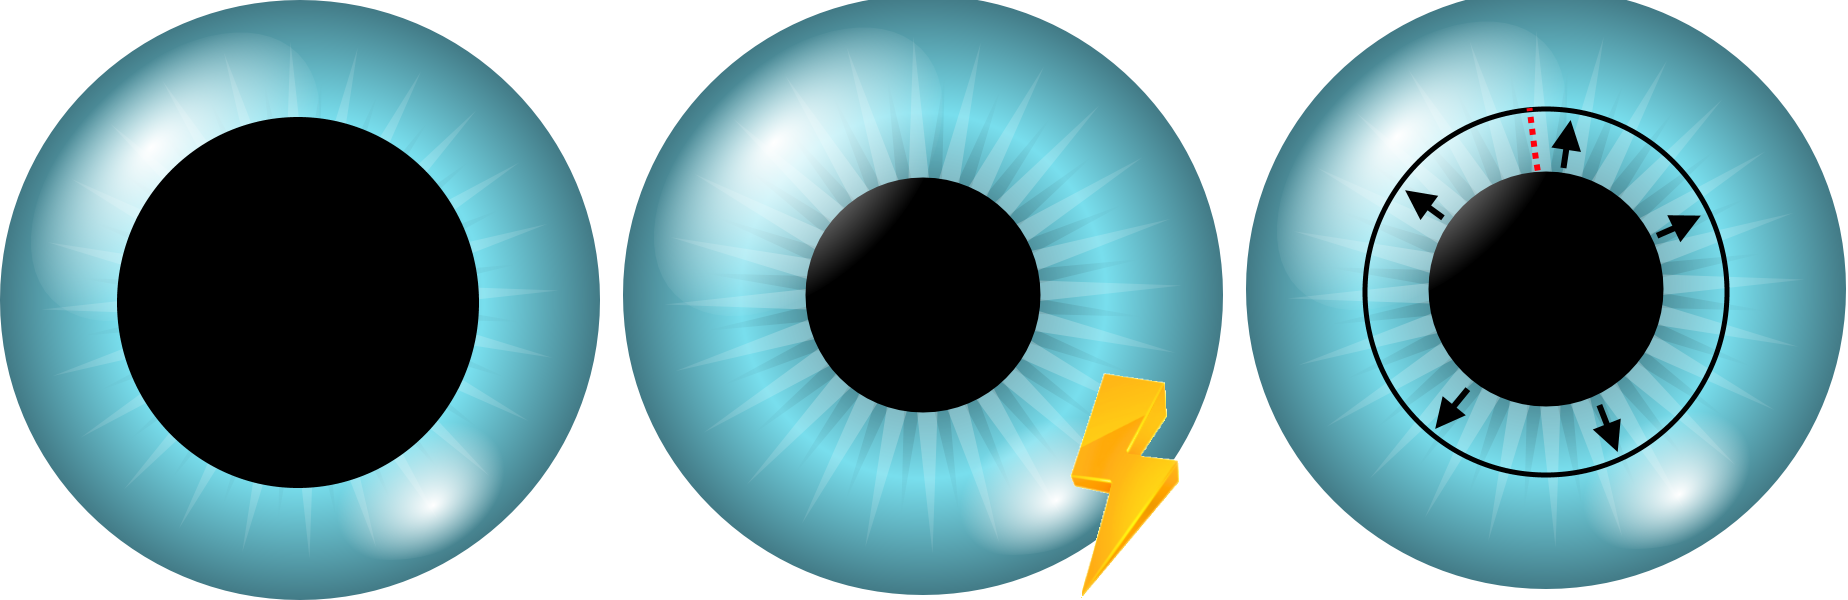
\includegraphics[width=\textwidth]{pupil-dilation}
\caption{Pupil reaktion.}
\end{subfigure}
~~~~
\begin{subfigure}[b]{0.45\textwidth}
	\centering
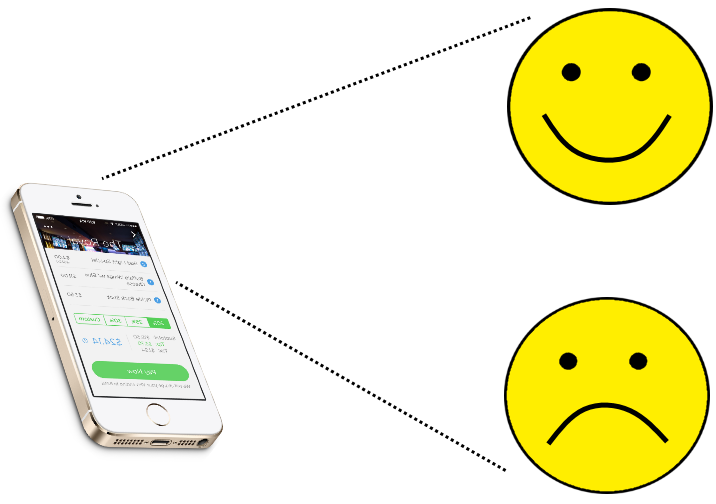
\includegraphics[width=\textwidth]{humoer}
\caption{Humør.}
\end{subfigure}
\caption{Idéer til brug af kameraet.}
\end{figure}

\end{frame}

\section{Accelerometer}
\begin{frame}[fragile]
\frametitle{Accelerometer}
\begin{columns}
\column[t]{5cm}
\begin{itemize}
\item Accelerometeret angiver en retning
\item Gyro sensoren angiver telefonens rotation
\item De kan bruges til evt. at se brugerens gangart
\item Eller til personens aktivitetsniveau
\end{itemize}

\column[t]{5cm}
\begin{figure}

\includegraphics[height=4cm]{red-to-green-gradient-thermometer}
\caption{En måde at visualisere ens aktivitetsniveau.}
\end{figure}
\end{columns}
\end{frame}



\section{Lokation}
\begin{frame}[fragile]
\frametitle{Lokation}
\begin{columns}
\column[t]{5cm}
\begin{itemize}
\item GPS sensoren giver en lokation
\item Kan vise hvor meget brugeren bevæger sig
\item Kan vise steder hvor brugere opholder sig mere end andre
\end{itemize}
\column[t]{5cm}
\begin{figure}
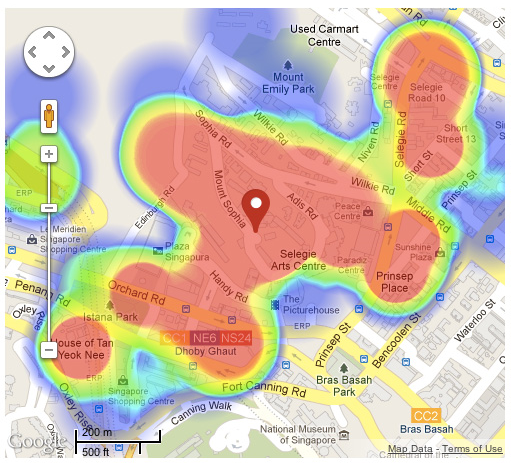
\includegraphics[height=4cm]{heatmap}
\caption{Et heatmap der viser hvor man opholder sig mest.}
\end{figure}
\end{columns}
\end{frame}



\section{Lyd}
\begin{frame}
\frametitle{Lyd}
\begin{itemize}
\item Mikrofonen kan bruges til at optage lyd
\item Optage telefonsamtaler
\item Optage når brugeren snakker vha. stemmegenkendelse
\item Parkinson syge er dårligere til at snakke
\item Andre sygdomme der har effekt på stemmen?
\end{itemize}
\end{frame}



\section{Lys}
\begin{frame}
\frametitle{Lys}
\begin{itemize}
\item Lyssensoren giver lysniveauets i lux
\item De fleste nyere telefoner har lyssensor
\item Kan bruges sammen med andre sensorer til at afgøre om en telefon er i lommen eller lignende
\end{itemize}
\end{frame}



\section{Opkald}
\begin{frame}
\frametitle{Opkald}
\begin{itemize}
\item Se på en brugers opkaldsoversigt
\item Antal opkald der er besvaret/ubesvaret
\item Telefonsamtalers varighed kan give en indikation
\item Hvilke personer man snakker med
\end{itemize}
\end{frame}



\section{Brug af mobil}
\begin{frame}
\frametitle{Brug af mobil}
\begin{itemize}
\item Logge hvilke applikationer der bliver brugt
\item Kan give et billede af brugerens social situation
\item Se om brugeren har sin telefon meget tændt når vedkommende befinder sig i sociale begivenheder i virkeligheden
\item Logge om der er ændringer i brugen af apps
\end{itemize}

\end{frame}



\section{Pulsmåler}
\begin{frame}[fragile]
\frametitle{Pulsmåler}
\begin{columns}
\column[t]{5cm}
\begin{itemize}
\item Kræver en pulsmåler
\item Der er ikke ret mange telefoner der har pulsmåler(endnu)
\item Vi er ikke sikre på at de er ret præcise
\item Man kan bruge en ekstern pulsmåler, fx et armbånd
\item Kan bruges til fx at måle brugerens aktivitetsniveau og evt. anfald(?)
\end{itemize}
\column[t]{5cm}
\begin{figure}
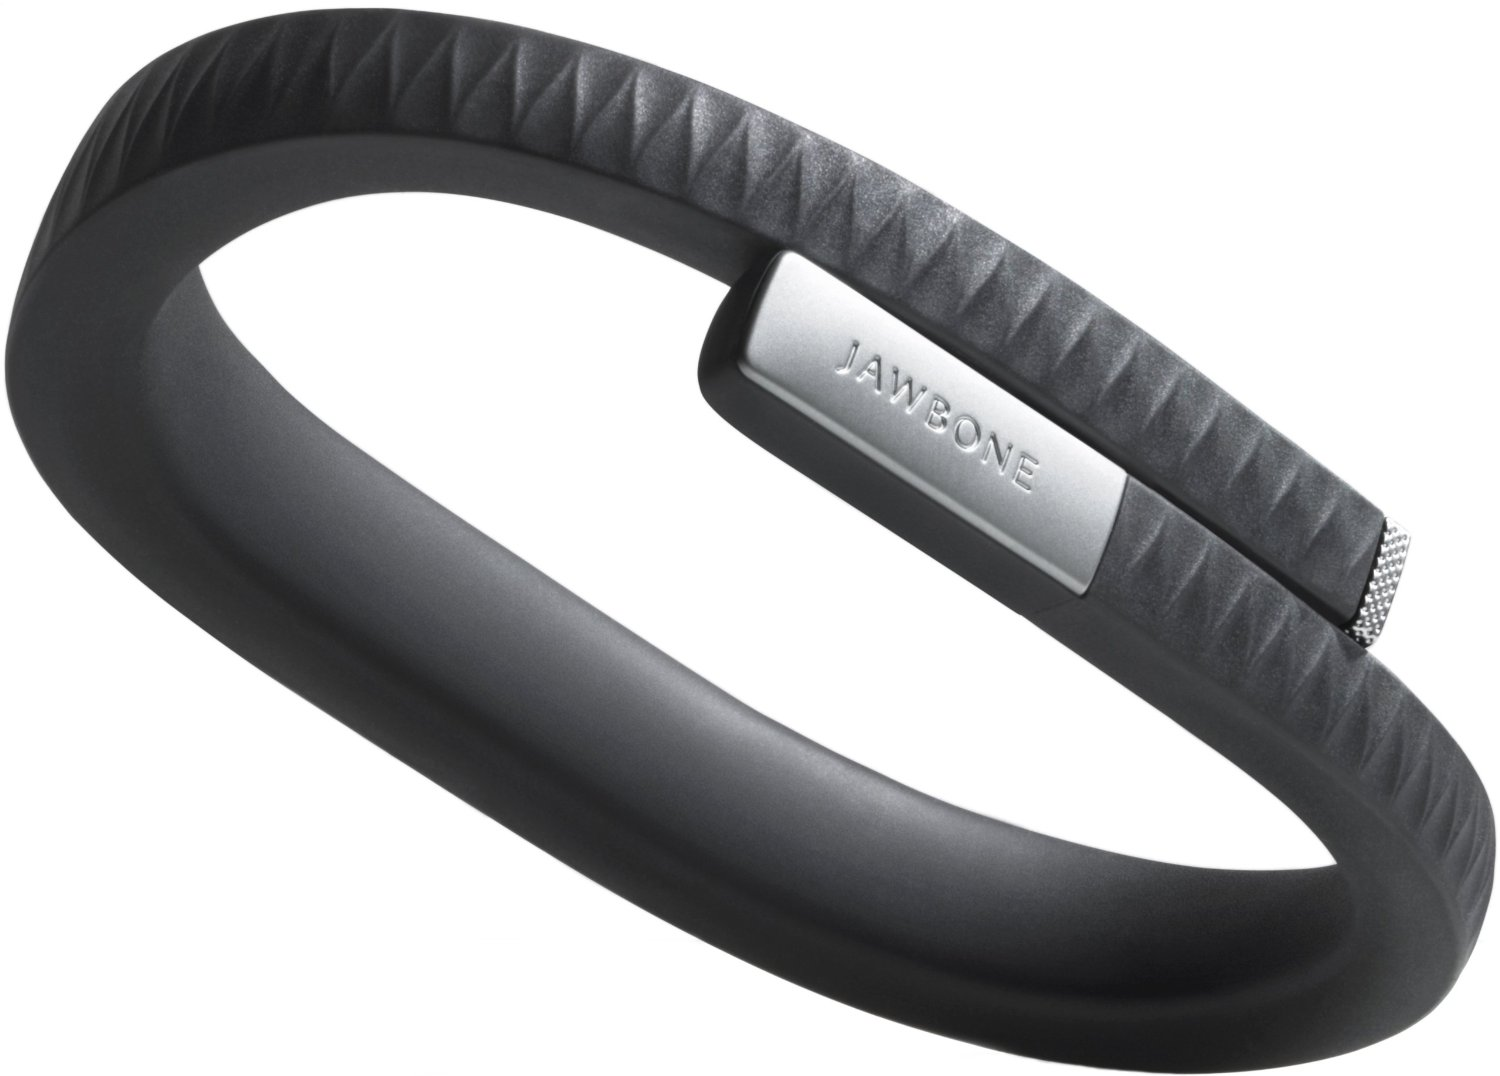
\includegraphics[height=4cm]{jaw_bone}
\caption{Et JawBone armbånd.}
\end{figure}
\end{columns}
\end{frame}


\section{Skærm}
\begin{frame}
\frametitle{Skærm}
\begin{itemize}
\item Det er muligt at vide hvor meget ens skærm er tændt og hvornår
\item Kan måske bruges til at estimere søvnlængde
\item ????
\end{itemize}
\end{frame}


\section{Galvanisk Hud Respons}
\begin{frame}
\frametitle{Galvanisk Hud Respons}
\begin{columns}
\column[t]{5cm}
\begin{itemize}
\item Kan måle hvor meget man sveder
\item Kræver en ekstern sensor
\item Kan måle om man er stresset
\item Stress er ofte første indikation på en depression
\item Kan fortælle personen at vedkommende skal lave noget afstressende
\item Kan bruges til at måle mængden af motion
\end{itemize}
\column[t]{5cm}
\begin{figure}
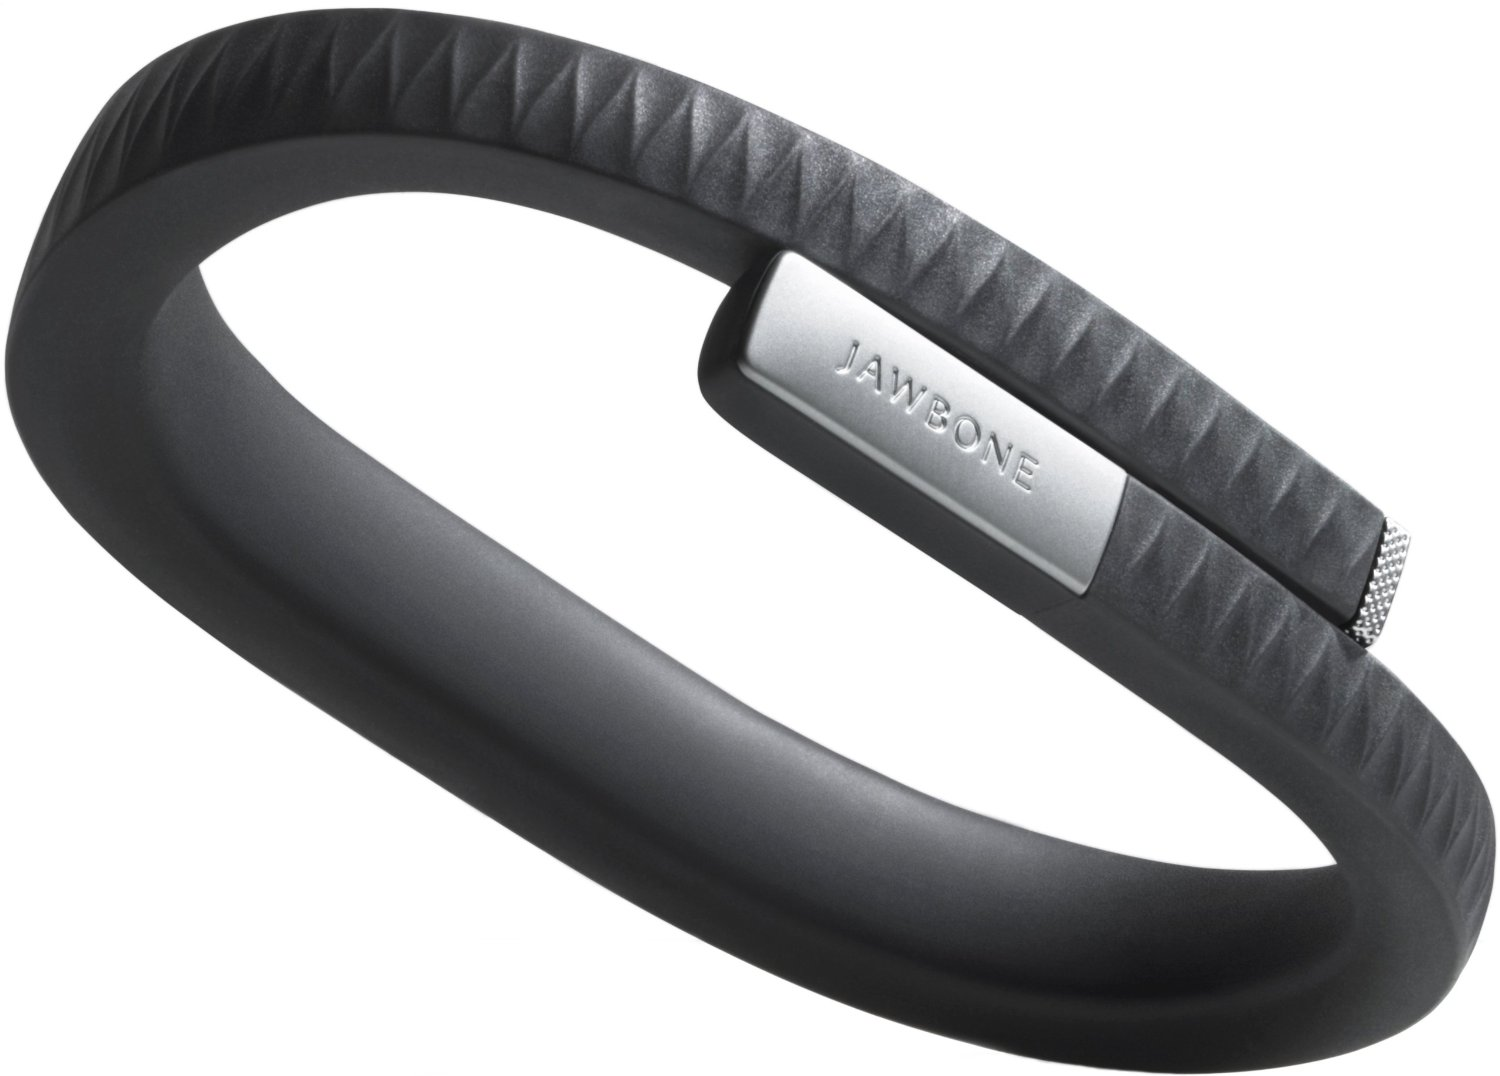
\includegraphics[height=4cm]{jaw_bone}
\caption{Et JawBone armbånd.}
\end{figure}
\end{columns}
\end{frame}


\section{Tastatur}
\begin{frame}
\frametitle{Tastatur}
\begin{itemize}
\item Man kan ikke få adgang til brugerens standard tastatur
\item For at få informationer fra tastatur bliver man nødt til at lave sit eget tastatur, som brugeren skal bruge
\item Se hvor lang tid det taer at skrive en sætning
\item Ordvalg
\item etc.
\end{itemize}
\end{frame}

\section{Tekstanalyse}
\begin{frame}
\frametitle{Tekstanalyse}
\begin{itemize}
\item Tekst fra: SMS og sociale medier(fx facebook beskeder)
\item Kigge på nøgleord som 'deprimeret'
\item Afsendelsestidspunkt, for at se om man er deprimeret i perioder
\item Se på om modtageren har en indflydelse
\item Længde af beskeder
\item Stemningsanalyse
\end{itemize}
\end{frame}

\begin{frame}
\frametitle{Tekstanalyse}
\begin{figure}
	\centering
	\begin{subfigure}[b]{0.3\textwidth}
		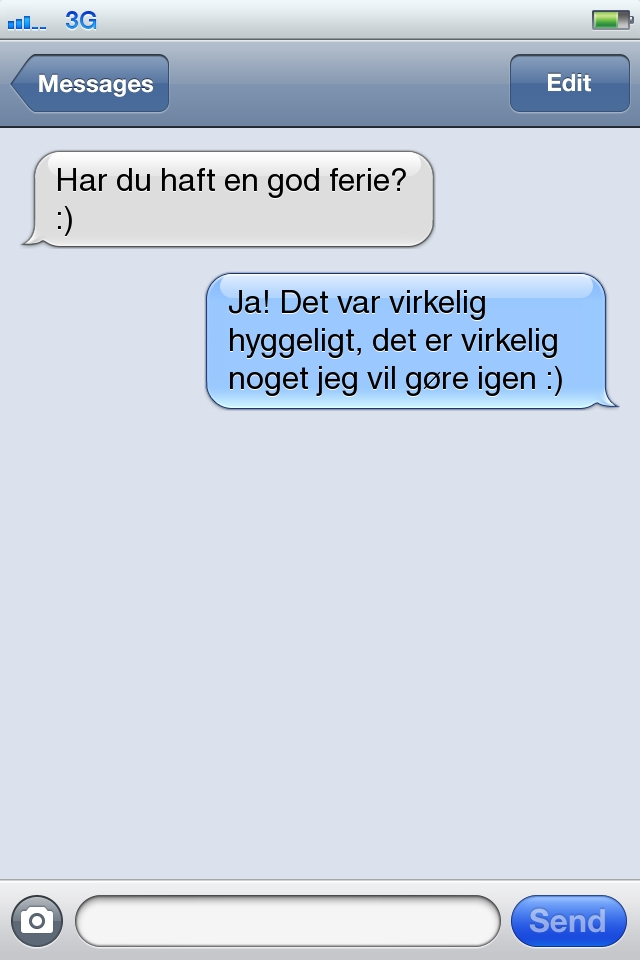
\includegraphics[width=\textwidth]{positiveSMS}
		\caption{Positiv SMS}
	\end{subfigure}
	~
	\begin{subfigure}[b]{0.3\textwidth}
		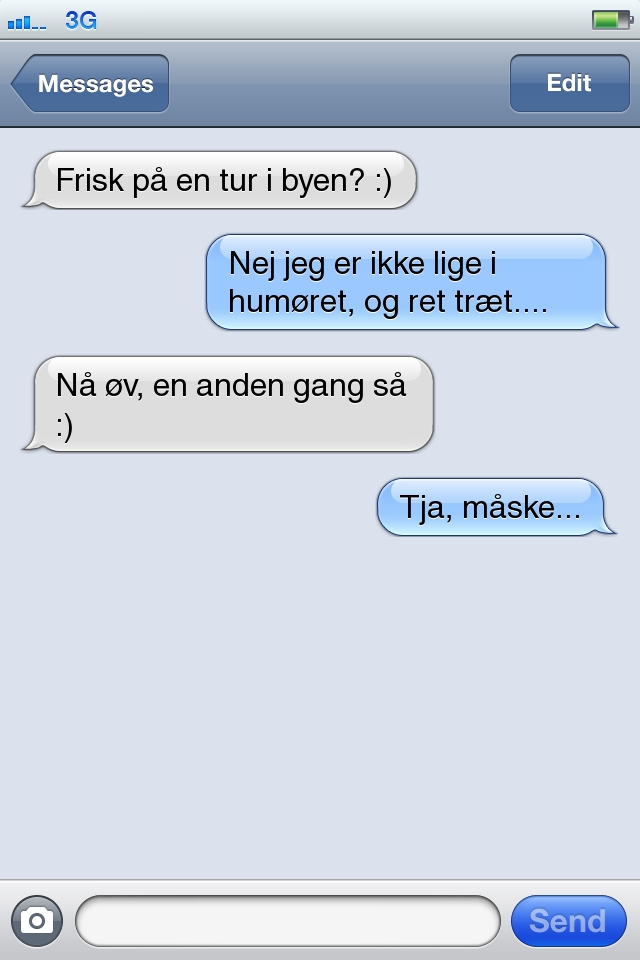
\includegraphics[width=\textwidth]{negativeSMS}
		\caption{Negativ SMS}
	\end{subfigure}
	\caption{Eksempler på SMS'er}
\end{figure}
\end{frame}